\newpage
\section{Aufbau und Durchführung}\label{sec:aufbau-und-durchfuehrung}
Der Versuch wird an einem Spektroskop durchgeführt, das wie folgt aufgebaut ist: Eine Lampe wirft durch eine Spaltöffnung einen Lichtstrahl durch ein Linsensystem, sodass ein paralleler Strahl entsteht, der ein drehbar gelagertes Flintglasprisma trifft. Das Licht vom Prisma kann dann durch ein Fernrohr beobachtet werden, an dem eine Winkelskala angebracht ist.

Der Versuch gliedert sich in zwei Abschnitte. Als erstes wird der Winkel~$\varphi$ zwischen den brechenden Prismenoberflächen bestimmt.
Dafür wird eine Kante des Prismas so ausgerichtet und fixiert, dass das Licht der HgCd-Lampe parallel auftrifft und an den beiden angrenzenden Oberflächen reflektiert wird. Der Aufbau ist in Abbildung~\ref{fig:prism} zu sehen.

\begin{figure}
  \centering
  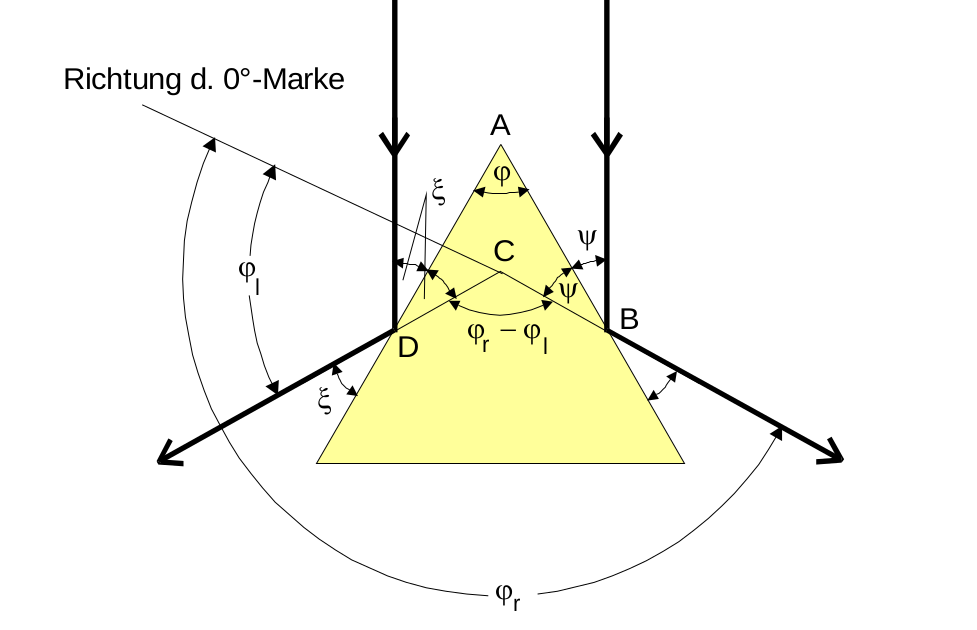
\includegraphics[width=0.4\textheight]{../figures/phi.png}
  \caption{Schematische Darstellung zur Messung des Winkels~$\varphi$ an der brechenden Kante eines Prismas. [Skript V402]}
\label{fig:prism}
\end{figure}

Nun wird das bewegliche Fernrohr so lange gedreht, bis die Spektrallinen des einen reflektierten Strahls genau im Fadenkreuz erscheinen und der Winkel notiert. Genauso verfährt man mit dem zweiten Satz an Spektrallinien. Auf diese Weise erhält man die zwei Winkel $\varphi_{\mathrm l}$ und $\varphi_{\mathrm r}$. Aus geometrischen Überlegungen erhält man für den Winkel~$\varphi$ der Kante
\begin{align}\label{equ:phi}
  \varphi = \frac{1}{2}(\varphi_{\mathrm r} - \varphi_{\mathrm l}) \; .
\end{align}

\par
Als zweites werden die Winkel $\eta_i$ der einzelnen Spektrallinien vermessen, die die Richtungsänderung des einfallenden Strahles charakterisieren.

Dazu wird ein symmetrischer Strahlengang hergestellt (siehe Abbildung~\ref{fig:sympris}). Dazu wird das Prisma so in den Lichtstrahl rotiert, dass Spiegelbild und gebrochenes Bild des Spaltes im Fernrohr unter dem gleichen Winkel erscheinen. Dann wird der Winkel einer Spektrallinie gemessen (bezüglich einer beliebigen, festen Stelle) und das Prisma so um die eigene Achse gedreht, dass spiegelsymmetrisch bezüglich des einfallenden Strahls zum ersten Zustand zu liegen kommt (siehe Abbildung~\ref{fig:spiegel}). Der Winkel, unter dem die gleichfarbige Spektrallinie erscheint wird wieder gemessen und die Differenz zum ersten Winkel $\Delta\Omega$ gebildet. Dadurch ergibt sich der Winkel $\eta$, unter dem der Strahl gebrochen wird zu
\begin{align}\label{equ:eta_}
	\eta = \pi - \Delta\Omega \;.
\end{align}
Dieses Verfahren wird für alle Spektrallinien wiederholt.

Aus den so gemessenen Winkeln ergibt sich mit dem Snelliusschen Brechungsgesetzt folgender Zusammenhang für den Brechungsindex:
\begin{align}\label{equ:brech}
	n = \frac{\sin(\eta/2+\varphi/2)}{\sin(\varphi/2)} \;.
\end{align}

\begin{figure}
  \centering
  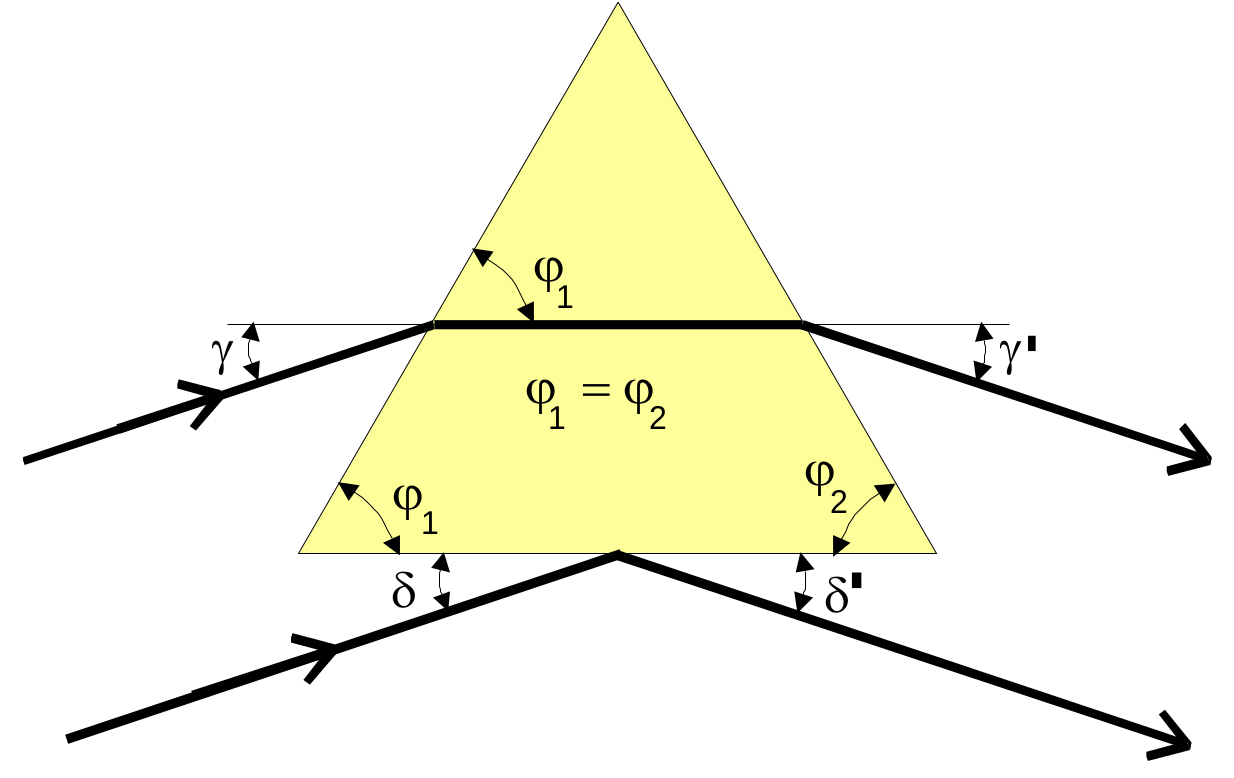
\includegraphics[width=0.4\textheight]{../figures/sym.png}
  \caption{Symmetrischer Strahlengang durch ein Prisma. [Skript V402]}
\label{fig:sympris}
\end{figure}

\begin{figure}
  \centering
  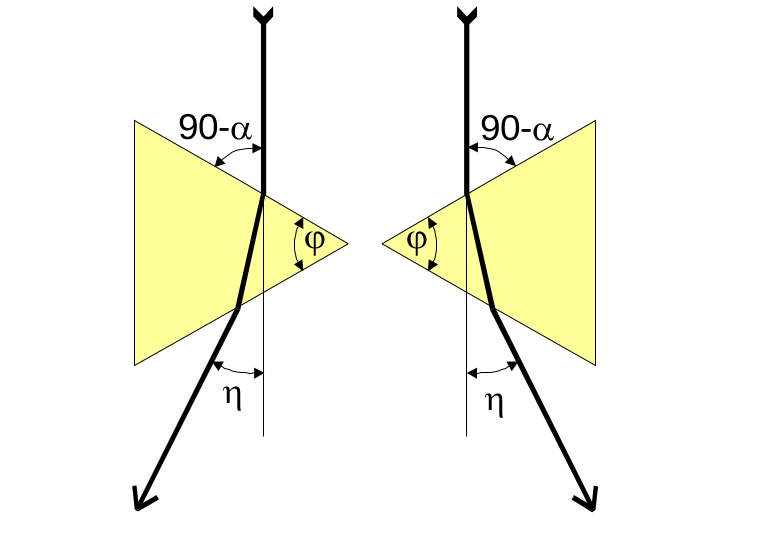
\includegraphics[width=0.4\textheight]{../figures/spiegel.png}
  \caption{Prisma wird ``gespiegelt''. [Skript V402]}
\label{fig:spiegel}
\end{figure}